% The harness loop for one target (driver.run_rounds + prove_top_spec.py).
% Build: pdflatex harness_loop.tex
%        pdftoppm -png -r 300 -singlefile harness_loop.pdf harness_loop
\documentclass[tikz,border=8pt]{standalone}
\usepackage[T1]{fontenc}
\usepackage{lmodern}
\renewcommand{\familydefault}{\sfdefault}
\usetikzlibrary{positioning,arrows.meta,calc,shapes.geometric}

\definecolor{frozen}{RGB}{210,225,250}
\definecolor{frozenline}{RGB}{50,90,170}
\definecolor{agent}{RGB}{214,240,214}
\definecolor{agentline}{RGB}{60,140,60}
\definecolor{fail}{RGB}{250,215,210}
\definecolor{failline}{RGB}{190,60,50}
\definecolor{warn}{RGB}{252,238,200}
\definecolor{warnline}{RGB}{190,140,30}
\definecolor{grey}{RGB}{235,235,235}
\definecolor{greyline}{RGB}{120,120,120}

\tikzset{
  box/.style={draw, rounded corners=3pt, line width=0.9pt, align=left,
              inner sep=6pt, font=\small},
  call/.style={-{Stealth[length=3mm]}, line width=1pt},
  lab/.style={font=\small\itshape, fill=white, inner sep=2pt},
}

\begin{document}
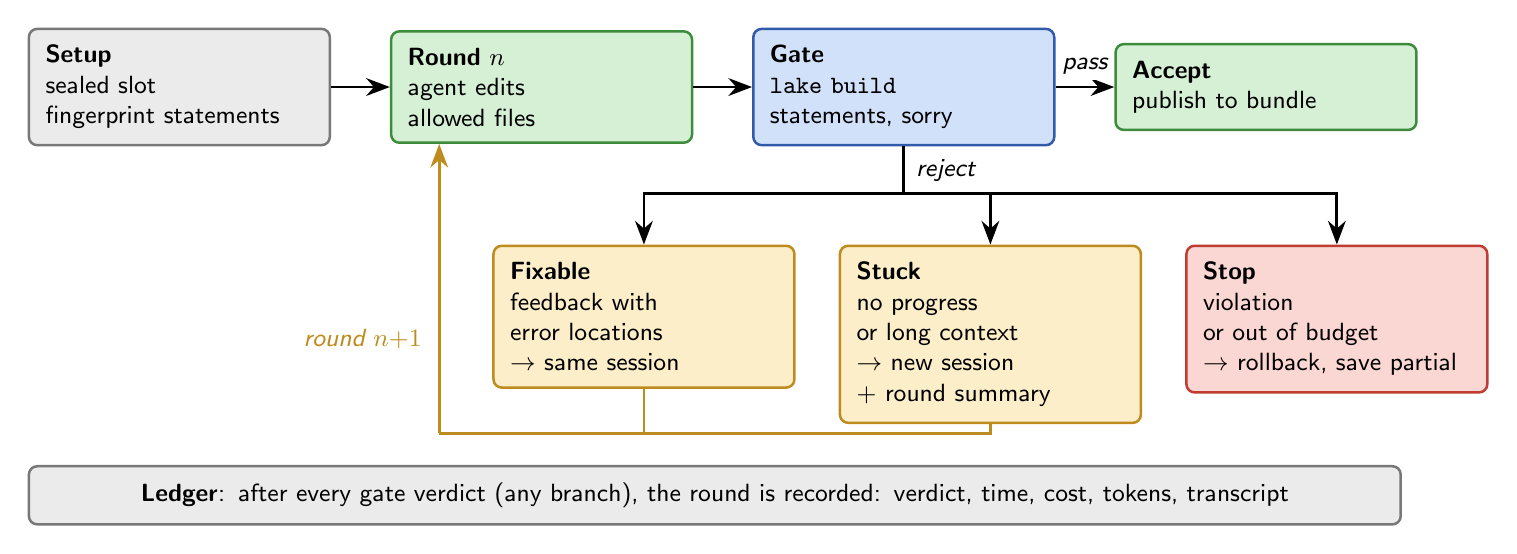
\begin{tikzpicture}

  %% main line
  \node[box, fill=grey, draw=greyline, text width=3.4cm] (setup) at (0,0) {%
    \textbf{Setup}\\ sealed slot\\ fingerprint statements};
  \node[box, fill=agent, draw=agentline, text width=3.4cm] (agent) at (4.6,0) {%
    \textbf{Round $n$}\\ agent edits\\ allowed files};
  \node[box, fill=frozen, draw=frozenline, text width=3.4cm] (gate) at (9.2,0) {%
    \textbf{Gate}\\ \texttt{lake build}\\ statements, sorry};
  \node[box, fill=agent, draw=agentline, text width=3.4cm] (acc) at (13.8,0) {%
    \textbf{Accept}\\ publish to bundle};

  \draw[call] (setup) -- (agent);
  \draw[call] (agent) -- (gate);
  \draw[call] (gate) -- node[lab, above=2pt] {pass} (acc);

  %% rejection branches
  \node[box, fill=warn, draw=warnline, text width=3.4cm, anchor=north] (fb) at (5.9,-2.0) {%
    \textbf{Fixable}\\ feedback with\\ error locations\\ $\to$ same session};
  \node[box, fill=warn, draw=warnline, text width=3.4cm, anchor=north] (rs) at (10.3,-2.0) {%
    \textbf{Stuck}\\ no progress\\ or long context\\ $\to$ new session\\ + round summary};
  \node[box, fill=fail, draw=failline, text width=3.4cm, anchor=north] (stop) at (14.7,-2.0) {%
    \textbf{Stop}\\ violation\\ or out of budget\\ $\to$ rollback, save partial};

  \coordinate (bus) at ($(gate.south)+(0,-0.6cm)$);
  \draw[line width=1pt] (gate.south) -- node[lab, right=2pt] {reject} (bus);
  \draw[call] (bus) -| (fb.north);
  \draw[call] (bus) -| (rs.north);
  \draw[call] (bus) -| (stop.north);

  %% back to the agent: round n+1
  \coordinate (ret) at (3.3,-4.4);
  \draw[line width=1pt, warnline] (fb.south) |- (ret);
  \draw[line width=1pt, warnline] (rs.south) |- (ret);
  \draw[call, warnline] (ret) -- (3.3,0 |- agent.south);
  \node[font=\small\itshape, text=warnline, anchor=east] at (3.2,-3.2) {round $n{+}1$};

  %% ledger band
  \node[box, fill=grey, draw=greyline, text width=17.0cm, anchor=north west, align=center]
      at ($(setup.west)+(0,-4.8cm)$) {%
    \textbf{Ledger}: after every gate verdict (any branch), the round is recorded: verdict, time, cost, tokens, transcript};
\end{tikzpicture}
\end{document}
